\documentclass[a4paper,10pt]{article}
\usepackage{hyperref}
\usepackage{float}
\usepackage{graphicx}
\usepackage{listings}

%%% Title
\title{Processo e Sviluppo Software: Assignment 3} 
\author{Ivo Junior Bettini - 806878, Umberto Cocca - 807191, \\Silvia Traversa - 816435\\
\href{https://gitlab.com/s.traversa/2019_assignment3_booksloan}{GitLab repository}}
\date{}

\begin{document}

\maketitle 

\section*{Applicazione}
L'applicazione BooksLoan permette agli utenti di visualizzare il catalogo di una biblioteca. Essi possono visualizzare sia le copie disponibili, ed eventualmente richiederne una in prestito, sia quelle non disponibili e prenotarle per quando ritorneranno presso la biblioteca.
E' inoltre possibili visualizzare le informazioni relative ad ogni singolo libro, quali l'autore o la presenza di sequel. 

\section*{Esecuzione dell'applicazione}
\subsection*{Preparazione database}
Prima di eseguire l'applicazione, è necessario importare i dati e la struttura del database, creato con MySQL.\\
Per effettuare questa operazione bisogna effettuare su MySQLWorkbench un Data Import del file \textit{DumpFinale} presente nella cartella \textit{dumps}. Successivamente, per permettere la connessione al database, è richiesta la modifica del file \textit{src/main/resources/application.properties} inserendo le proprie credenziali MySQL nei campi spring.datasource.username e spring.datasource.password, come illustrato nella figura.\\
\begin{figure}[H]
	\centering
	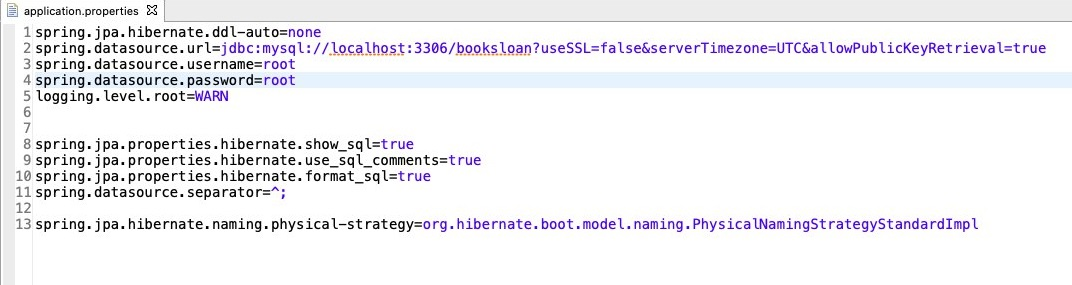
\includegraphics[width=1\linewidth]{images/properties}
\end{figure}

\subsection*{Applicazione}

Per far partire l'applicazione, dopo aver clonato il repository, esegurie i seguenti comandi

\begin{lstlisting}[language=bash]
	mvnw clean package spring-boot:repackage
\end{lstlisting}

\begin{lstlisting}[language=bash]
	java target/BooksLoan-1.jar
\end{lstlisting}

L'applicazione sarà disponibile all'indirizzo \href{http://localhost:8080}{http://localhost:8080}.\\

Per accedere alle funzionalità dell'applicazione è rischiesto un log-in, che è possibile effettuare con tre diversi account, rappresentativi di categorie che verrano spiegate nel dettaglio in seguito:

\begin{itemize}
	\item \textbf{amministratore con contratto a tempo indeterminato:}
\begin{lstlisting}[language=bash]
    username: 123 password: 1234
\end{lstlisting}
	\item \textbf{amministratore con contratto a tempo determinato:}
\begin{lstlisting}[language=bash]
    username: 456 password: 4567
\end{lstlisting}
	\item \textbf{cliente:}
\begin{lstlisting}[language=bash]
    username: 321 password: 1234
\end{lstlisting}
\end{itemize}

\section*{Schema E-R}

\begin{figure}[H]
	\centering
	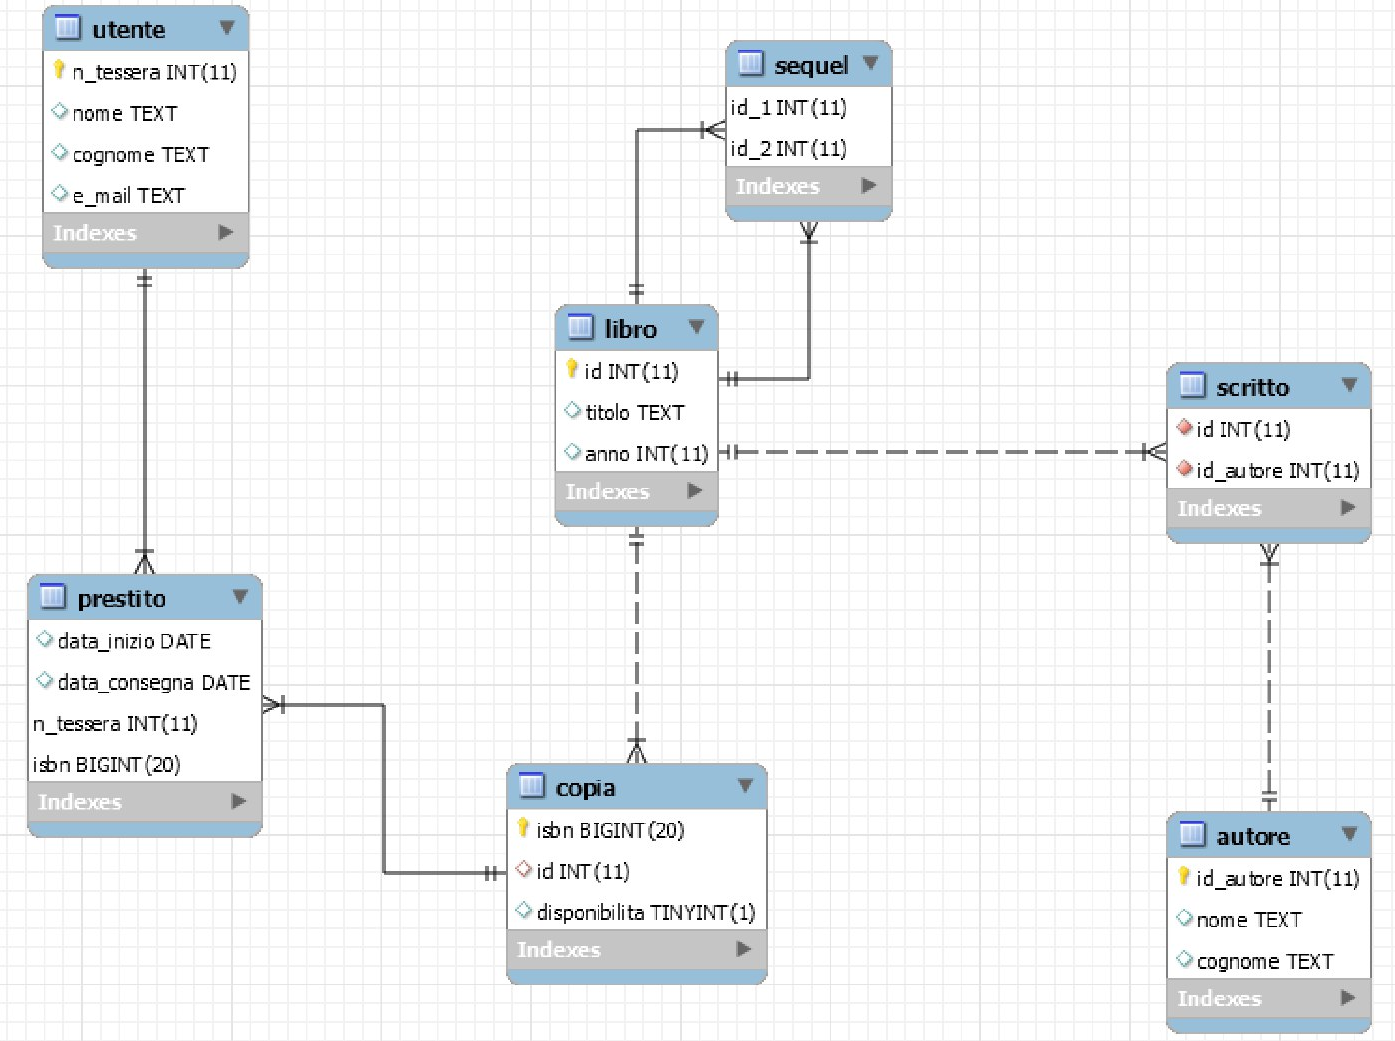
\includegraphics[width=0.7\linewidth]{images/ERdiagram}
	\caption[Schema ER]{Schema ER}
	\label{fig:re}
\end{figure}

Le entità utilizzate nel nostro progetto sono così descritte:

\begin{itemize}
	\item Utente: descrive la persona registrata e utilizzatrice del sito
	\item Libro: elemento che compone la nostra libreria online
	\item Copia: insieme di diverse edizioni di un libro
	\item Autore: colui che ha scritto uno o più libri
\end{itemize}

Esse sono messe in relazione da:
\begin{itemize}
	\item Prestito: entità che relaziona utente con copia
	\item Sequel: entità che mette in relazione un libro con se stesso
	\item Scritto: entità che mette in relazione autore con libro
\end{itemize}

In particolare:
\begin{itemize}
	\item Un utente può effettuare tanti prestiti ma richiedere una sola copia di un libro alla volta
	\item Un libro può essere presente in più copie o nessuna
	\item Una copia può trovarsi in due stati, disponibile o non disponibile (in quest'ultimo caso non può essere presa in prestito)
	\item Un libro può essere in relazione ad un altro in quanto suo sequel
	\item Un libro può essere scritto da uno o più autori e un autore può scrivere uno o più libri
\end{itemize}

All’interno dell’applicazione è presente un package di controller che permette le operazioni di CRUD tra le classi sopra citate.

\section*{BooksLoan}
Per poter accedere all’applicazioni bisogna obbligatoriamente essere registrati, esistono due tipi di utente:

\begin{itemize}
	\item Amministratore (che a sua volta viene distinto in base alla tipologia di contratto)
	\item Cliente
\end{itemize}

Il cliente, una volta effettuato il log-in, ha a disposizione l'elenco dei libri del catalogo della biblioteca. Può visualizzare se sono presenti delle copie disponibili di un determinato libro ed eventualmente prenderla in prestito.
Inoltre può visualizzare i suoi prestiti in corso e restituire una copia.

L'amministratore si divide in due tipologie: quello con un contratto a tempo indeterminato e quello con un contratto a tempo determinato. 
Il primo ha la possibilità di effettuare ogni tipo di operazione: può eliminare, aggiungere, modificare libri e copie, impostare i sequel di un libro e aggiungere l'autore relativo.
Un amministratore con contratto a tempo determinato, invece, non ha la facoltà di effettuare operazioni di cancellazione.

\end{document}